% Provenance (never printed): see sources/outline_sources.md (Year 1: field
% notebook, compass-clinometer, hand lens, sampling, polarising microscope and
% thin sections, safety). The readings of the Varden east limb are simulated
% in figdata/bachelor-1/attitude_stats.py (seed 83, errors of 3 degrees);
% problem values in the Book 3 scratch calculator calc/ch06.py.
\chapter{Métodos de campo y de laboratorio I}\label{ch:b1:field-lab-methods-1}

Un geólogo que cartografía las colinas de Varden lleva poco equipo: una libreta, un lápiz, un
receptor de satélite, una brújula-clinómetro, una lupa de mano y unas cuantas bolsas de muestras.
Con ellos fija dónde está, mide la \omterm{def:b1:geological-maps:attitude}{actitud} de los estratos, nombra las rocas y trae las muestras que
el laboratorio cortará, pulirá y observará al microscopio. Cada número de los capítulos anteriores ---una
\omterm{def:b1:geological-maps:attitude}{actitud} en un mapa, un \omterm{def:b1:geological-maps:attitude}{buzamiento} en un corte--- empezó como una lectura de este tipo, con su propio
error. Este capítulo describe cómo los profesionales hacen estas observaciones, y cómo se promedian las
lecturas repetidas y su dispersión se convierte en una incertidumbre. Termina con una temporada de
lecturas en el flanco oriental del \omterm{def:b1:geological-maps:fold}{anticlinal} de Varden.

\begin{recall}
La \omterm{def:b1:geological-maps:attitude}{actitud} de un plano se escribe \omterm{def:b1:geological-maps:attitude}{dirección de buzamiento}/\omterm{def:b1:geological-maps:attitude}{buzamiento}, como $081/12$, o como un \omterm{def:b1:geological-maps:attitude}{rumbo}
según la regla de la mano derecha con un \omterm{def:b1:geological-maps:attitude}{buzamiento} (\cref{ch:b1:geological-maps}). La declinación
magnética es el ángulo entre el norte geográfico y la dirección en la que apunta la aguja de una
brújula (física, año 11). Los minerales se reconocen en la mano por su brillo, su exfoliación, su
dureza y su color (libro 2, año 11). La media y la desviación típica de un conjunto de números resumen
su centro y su dispersión (matemáticas).
\end{recall}

\section{El cuaderno y el mapa}

\begin{definition}[Estación de campo, cuaderno de campo]\label{def:b1:field-lab-methods-1:station}
Una \emph{estación de campo}\index{estación de campo} es un lugar numerado donde un geólogo hace y
anota observaciones: su posición, las rocas vistas, su \omterm{def:b1:geological-maps:attitude}{actitud} y las muestras tomadas. El
\emph{cuaderno de campo}\index{cuaderno de campo} es el registro encuadernado de las estaciones, en el
orden en que se visitaron, con sus números, croquis y medidas, escritos en el acto.
\end{definition}

El cuaderno es el registro primario: lo que no se anota en la estación se pierde, y un mapa dibujado
por la tarde vale solo lo que valen las notas en que se basa. Cada estación tiene un número que
aparece en el mapa de campo, en el cuaderno y en cada bolsa de muestra tomada allí. Un croquis muestra
lo que una lista de números no puede ---cómo se encuentran dos unidades, hacia dónde están las capas
más jóvenes, dónde se tomó una lectura en una superficie plegada--- y registra su escala y su
orientación. Los hechos y las interpretaciones se mantienen separados: ``caliza sobre lutita, contacto
neto'' es una observación; ``\omterm{def:b1:cross-sections:unconformity}{discordancia}'' es una inferencia, y se escribe como tal.

\begin{inthefield}[Un día de cartografía]
% ledger: gps:smartphone-accuracy, gps:high-end
\begin{minipage}[t]{0.58\linewidth}\vspace{0pt}
Un geólogo que cartografía plantea una travesía transversal al \omterm{def:b1:geological-maps:attitude}{rumbo}, de modo que encuentre cada
unidad a su vez, y se detiene allí donde aparece un contacto, un cambio de roca o una superficie
medible. En cada estación escribe el número y la posición, dibuja lo que ve, mide \omterm{def:b1:geological-maps:attitude}{actitudes} y anota
las muestras. Las posiciones proceden de un receptor de satélite: un receptor corriente, como el de un
teléfono inteligente, tiene normalmente una precisión de unos \qty{4.9}{m} con cielo despejado, peor
junto a acantilados y árboles, mientras que los receptores de topografía que usan dos frecuencias o
servicios de corrección llegan a unos pocos centímetros. A una escala de mapa de 1:10\,000,
\qty{4.9}{m} son medio milímetro: un receptor corriente basta para cartografiar, pero no para medir el
lento movimiento del terreno (\cref{ch:b1:plate-kinematics}).
\end{minipage}\hfill
\begin{minipage}[t]{0.39\linewidth}\vspace{0pt}
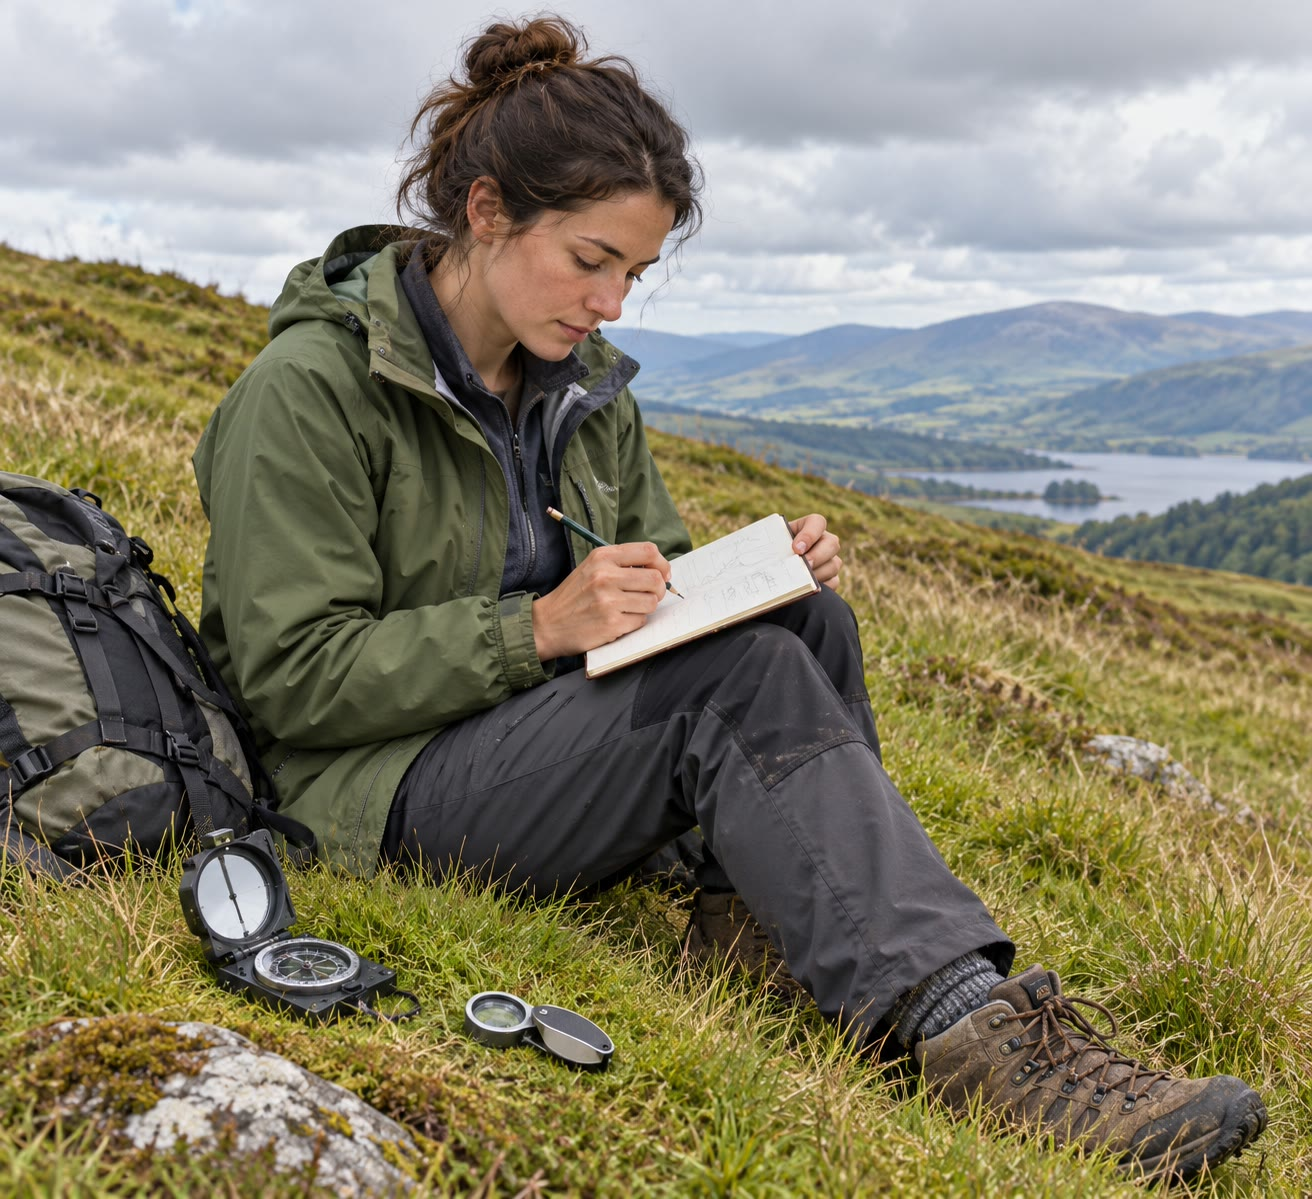
\includegraphics[width=\linewidth]{images/book3/ai/b1-field-notebook.jpg}
\end{minipage}
\end{inthefield}

\section{Medir orientaciones}

La \omterm{def:b1:geological-maps:attitude}{actitud} de un plano ---un estrato, una falla, una diaclasa--- se mide con una brújula-clinómetro:
una brújula magnética para leer \omterm{def:b1:spherical-astronomy:horizontal}{acimutes}, y una plomada o un nivel para leer ángulos respecto de la
horizontal. Su borde se apoya según el \omterm{def:b1:geological-maps:attitude}{rumbo} de la superficie para leer el \omterm{def:b1:geological-maps:attitude}{rumbo}, o el instrumento se
coloca sobre la superficie según su línea de máxima pendiente para leer el \omterm{def:b1:geological-maps:attitude}{buzamiento} y, a partir del
\omterm{def:b1:spherical-astronomy:horizontal}{acimut} de esa línea, la \omterm{def:b1:geological-maps:attitude}{dirección de buzamiento}.

\begin{omfigure}
\begin{tikzpicture}[font=\scriptsize]
% (a) plan view
\begin{scope}
\fill[icsJurassic!25] (0,0) -- (3.6,0.5) -- (3.9,2.9) -- (0.3,2.4) -- cycle;
\draw (0,0) -- (3.6,0.5) -- (3.9,2.9) -- (0.3,2.4) -- cycle;
\draw[omDef, thick] (0.4,1.55) -- (3.5,1.98);
  \node[omDef, above, rotate=8, fill=icsJurassic!25, inner sep=1pt] at (0.95,1.65) {línea de rumbo};
% compass box laid along the strike line
\begin{scope}[shift={(2.5,1.84)}, rotate=8]
\draw[fill=white] (-0.6,0) rectangle (0.6,0.32);
\draw (0,0.16) circle (0.12);
\end{scope}
\draw[omThm, thick, -{Stealth[length=2mm]}] (1.6,1.71) -- (1.75,0.62);
\node[omThm, right, fill=icsJurassic!25, inner sep=1pt] at (1.78,0.85) {dirección de buzamiento};
\node[below, align=center] at (1.95,-0.15) {(a) vista en planta: el borde de\\ la brújula según el rumbo};
\draw[->] (4.3,1.6) -- (4.3,2.4) node[above] {N};
\end{scope}
% (b) side view, vertical section along the dip direction
\begin{scope}[xshift=5.8cm]
\fill[icsJurassic!25] (0,1.6) -- (3.6,0.2) -- (3.6,-0.3) -- (0,-0.3) -- cycle;
\draw[thick] (0,1.6) -- (3.6,0.2);
% clinometer resting on the surface
\begin{scope}[shift={(2.5,0.6278)}, rotate=-21.25]
\draw[fill=white] (-0.75,0) rectangle (0.75,0.3);
\draw (0,0.15) circle (0.11);
\draw[black!70] (0,0.15) -- ++(-68.75:0.11);
\end{scope}
% dip angle at the lower end of the surface
\coordinate (P) at (0.7,1.3278);
\draw[black!60] (P) -- ++(1.6,0) node[right] {horizontal};
\draw[omThm] ($(P)+(1.1,0)$) arc[start angle=0, end angle=-21.25, radius=1.1];
\node[omThm] at ($(P)+(0.9,-0.15)$) {$\delta$};
\node[below, align=center] at (1.8,-0.35) {(b) corte según la dirección de buzamiento:\\ el clinómetro sobre la línea de máxima pendiente};
\end{scope}
\end{tikzpicture}

{\small Medición de una \omterm{def:b1:geological-maps:attitude}{actitud} (esquema). (a) El borde de la brújula apoyado horizontalmente sobre
el estrato da el \omterm{def:b1:geological-maps:attitude}{rumbo}; la \omterm{def:b1:geological-maps:attitude}{dirección de buzamiento} es perpendicular a él, cuesta abajo. (b) Colocado
sobre su borde según la línea de máxima pendiente, el clinómetro da el \omterm{def:b1:geological-maps:attitude}{buzamiento} $\delta$.}
\end{omfigure}

Una recta ---un \omterm{def:b1:geological-maps:fold}{eje de pliegue}, una estría sobre una superficie de falla, el eje largo de los
cantos rodados--- tiene una orientación propia.

\begin{definition}[Dirección e inmersión]\label{def:b1:field-lab-methods-1:trend-plunge}
La \emph{dirección}\index{dirección (de una recta)} de una recta es el \omterm{def:b1:spherical-astronomy:horizontal}{acimut} de su proyección
horizontal, medido hacia el extremo de la recta que apunta hacia abajo. Su \emph{inmersión}\index{inmersión}
es el ángulo entre la recta y la horizontal, medido en el plano vertical que la contiene. Una recta
con inmersión de \ang{20} hacia \ang{015} se escribe $20\to015$.
\end{definition}

Una recta de \omterm{def:b1:field-lab-methods-1:trend-plunge}{dirección} $t$ e \omterm{def:b1:field-lab-methods-1:trend-plunge}{inmersión} $p$ tiene, en las componentes este, norte y arriba, el vector unitario hacia abajo
$(\cos p\sin t, \cos p\cos t, -\sin p)$; una recta contenida en
un plano de \omterm{def:b1:geological-maps:attitude}{dirección de buzamiento} $\alpha$ y \omterm{def:b1:geological-maps:attitude}{buzamiento} $\delta$ se hunde con el \omterm{def:b1:cross-sections:apparent-dip}{buzamiento aparente}
de ese plano en el plano vertical de \omterm{def:b1:spherical-astronomy:horizontal}{acimut} $t$, así que $\tan p = \tan\delta\cos(\alpha - t)$
(\cref{thm:b1:cross-sections:apparent-dip}).

\subsection{La declinación magnética}

Una aguja de brújula apunta al norte magnético, no al norte geográfico; el ángulo entre ambos es la
declinación magnética, que se cuenta positiva cuando el norte magnético está al este del norte
geográfico. Los mapas y las \omterm{def:b1:geological-maps:attitude}{actitudes} de este libro usan \omterm{def:b1:spherical-astronomy:horizontal}{acimutes} geográficos.

\begin{method}[Corrección del acimut de una brújula]\label{met:b1:field-lab-methods-1:declination}
\begin{enumerate}
  \item Búsquese la declinación magnética $D$ para el lugar y la fecha, en un modelo del campo
        terrestre (positiva al este, negativa al oeste).
  \item Súmese a cada \omterm{def:b1:spherical-astronomy:horizontal}{acimut} leído en la brújula: \omterm{def:b1:spherical-astronomy:horizontal}{acimut} geográfico $=$ \omterm{def:b1:spherical-astronomy:horizontal}{acimut} magnético $+ D$,
        módulo \ang{360}.
  \item No se corrijan los \omterm{def:b1:geological-maps:attitude}{buzamientos} ni las \omterm{def:b1:field-lab-methods-1:trend-plunge}{inmersiones}: se miden respecto de la horizontal, con la
        gravedad, no con la aguja.
\end{enumerate}
La mayoría de las brújulas de campo pueden ajustarse para sumar $D$ mecánicamente; el ajuste, y el año
para el que se hizo, se anotan en el cuaderno.
\end{method}

\begin{dated}{2026}
% ledger: noaa:wmm-edinburgh, noaa:wmm-reykjavik, noaa:wmm-anchorage, noaa:wmm-wellington
El 1 de enero de 2026, el Modelo Magnético Mundial (versión 2025) da la declinación magnética como
\ang{-0.47} (oeste) en Edimburgo, con una variación de \ang{+0.20} por año; \ang{-11.28} en Reikiavik,
con una variación de \ang{+0.30} por año; \ang{+14.20} (este) en Anchorage, con una variación de
\ang{-0.28} por año; y \ang{+23.23} en Wellington. Un geólogo que olvidara la corrección en Wellington
desplazaría cada \omterm{def:b1:spherical-astronomy:horizontal}{acimut} en más de \ang{23}; uno que reutilizara un ajuste de Edimburgo de diez años
antes arrastraría un error de unos \ang{2}.
\end{dated}

\subsection{Lecturas repetidas}

Una sola lectura de un plano de estratificación lleva errores: la superficie nunca es un plano
perfecto, el instrumento no está perfectamente colocado y la lectura se redondea al grado. Por eso el
geólogo mide varias veces la misma superficie, o varias superficies del mismo flanco, y promedia.
Promediar \omterm{def:b1:spherical-astronomy:horizontal}{acimutes} requiere cuidado: las lecturas \ang{355} y \ang{005} describen direcciones separadas
\ang{10}, pero su media aritmética, \ang{180}, apunta en sentido contrario. La media correcta trabaja con
vectores.

\begin{definition}[Orientación media (media vectorial)]\label{def:b1:field-lab-methods-1:mean-orientation}
Para un plano de \omterm{def:b1:geological-maps:attitude}{dirección de buzamiento} $\alpha$ y \omterm{def:b1:geological-maps:attitude}{buzamiento} $\delta$, sea
\[
  \vec n = (\sin\delta\sin\alpha,\ \sin\delta\cos\alpha,\ \cos\delta)
\]
su normal unitaria hacia arriba, en componentes este, norte y arriba. La \emph{orientación media}\index{orientación media}
(o \emph{media vectorial}) de $N$ lecturas de normales $\vec n_1, \dots, \vec n_N$ es el plano cuya normal es
$\vec m = \vec S/\|\vec S\|$, donde $\vec S = \sum_i \vec n_i$ es su resultante; $\bar R = \|\vec S\|/N$ es la
\emph{longitud resultante media}. El \omterm{def:b1:geological-maps:attitude}{buzamiento} medio y la \omterm{def:b1:geological-maps:attitude}{dirección de buzamiento} media son
$\bar\alpha = \operatorname{atan2}(S_E, S_N)$ y $\bar\delta = \arccos(S_U/\|\vec S\|)$.
\end{definition}

Que $\vec n$ es la normal se sigue de \cref{ch:b1:geological-maps}: el plano
$z = -\tan\delta\,(x\sin\alpha + y\cos\alpha)$ tiene la normal hacia arriba
$(\tan\delta\sin\alpha, \tan\delta\cos\alpha, 1)$, cuya longitud es $1/\cos\delta$.

\begin{proposition}[La media vectorial es la dirección más próxima]\label{prop:b1:field-lab-methods-1:vector-mean}
Entre todos los vectores unitarios $\vec u$, la normal media $\vec m$ maximiza
$\sum_i \vec n_i\cdot\vec u = \sum_i \cos\theta_i(\vec u)$, donde
$\theta_i(\vec u)$ es el ángulo entre $\vec n_i$ y $\vec u$; equivalentemente,
minimiza $\sum_i \|\vec n_i - \vec u\|^2$. Además
\[
  \bar R = \frac1N\sum_i \cos\theta_i, \qquad \theta_i = \theta_i(\vec m),
\]
así que $0 < \bar R \le 1$, con $\bar R = 1$ solo si todas las lecturas coinciden, y, cuando la dispersión
es pequeña, el ángulo cuadrático medio entre las lecturas y su media es
\[
  \theta_{\text{rms}} \approx \sqrt{2(1 - \bar R)} \quad\text{(radianes)}.
\]
\end{proposition}

\begin{proof}
$\sum_i \vec n_i\cdot\vec u = \vec S\cdot\vec u \le \|\vec S\|$ por la desigualdad de Cauchy--Schwarz,
con igualdad exactamente cuando $\vec u = \vec m$. Como $\|\vec n_i - \vec u\|^2 = 2 - 2\,\vec n_i\cdot\vec u$,
los dos problemas son el mismo. Con $\vec u = \vec m$ se alcanza la cota:
$\|\vec S\| = \sum_i\cos\theta_i$, que es la fórmula de $\bar R$. Por último, $\cos\theta \approx 1 - \theta^2/2$
para $\theta$ pequeño, así que $1 - \bar R \approx
\frac1N\sum_i\theta_i^2/2 = \theta_{\text{rms}}^2/2$.
\end{proof}

¿Cómo mueven los errores de los dos ángulos a la normal? Derivando $\vec n$,
\[
  \frac{\partial\vec n}{\partial\delta} = (\cos\delta\sin\alpha,\ \cos\delta\cos\alpha,\ -\sin\delta),
  \qquad
  \frac{\partial\vec n}{\partial\alpha} = (\sin\delta\cos\alpha,\ -\sin\delta\sin\alpha,\ 0):
\]
la primera tiene longitud 1, la segunda longitud $\sin\delta$, y las dos son perpendiculares. Pequeños
errores $\Delta\delta$ y $\Delta\alpha$ hacen girar, por tanto, la normal el ángulo
\[
  \Delta\theta \approx \sqrt{\Delta\delta^2 + \sin^2\delta\,\Delta\alpha^2}.
\]
Sobre un estrato de \omterm{def:b1:geological-maps:attitude}{buzamiento} suave, un error en la \omterm{def:b1:geological-maps:attitude}{dirección de buzamiento} apenas cambia el plano: en un
estrato que buza \ang{12}, un error de \ang{3} en la \omterm{def:b1:geological-maps:attitude}{dirección de buzamiento} hace girar el plano solo
$3\sin\ang{12} = \ang{0.6}$. Lo inverso es la dificultad del geólogo de campo: la \omterm{def:b1:geological-maps:attitude}{dirección de buzamiento} de
un estrato suave está mal fijada por su plano, y pequeñas ondulaciones de la superficie la dispersan mucho.
El error típico de la media de $N$ lecturas independientes, de desviación típica $s$, es $s/\sqrt N$
(matemáticas): para reducirlo a la mitad hacen falta cuatro veces más lecturas.

\begin{omfigure}
\begin{tikzpicture}
\begin{axis}[name=dd, width=0.47\linewidth, height=4.6cm, ybar, bar width=0.8,
  xmin=72.5, xmax=88.5, ymin=0, ymax=8.5, ytick={0,2,4,6,8},
  tick label style={font=\scriptsize}, label style={font=\small},
  xlabel={dirección de buzamiento (\si{\degree})}, ylabel={medidas}]
\addplot[fill=icsJurassic!40, draw=black] table[x=value, y=count] {figdata/out/bachelor-1-attitude_stats-hist-dd.dat};
\draw[omThm, thick] (axis cs:80.84,0) -- (axis cs:80.84,8.5);
\draw[omThm, densely dashed] (axis cs:77.91,0) -- (axis cs:77.91,8.5);
\draw[omThm, densely dashed] (axis cs:83.77,0) -- (axis cs:83.77,8.5);
\end{axis}
\begin{axis}[at={(dd.east)}, anchor=west, xshift=1.1cm, width=0.47\linewidth, height=4.6cm,
  ybar, bar width=0.8, xmin=5.5, xmax=18.5, ymin=0, ymax=8.5, ytick={0,2,4,6,8},
  tick label style={font=\scriptsize}, label style={font=\small},
  xlabel={buzamiento (\si{\degree})}]
\addplot[fill=icsJurassic!40, draw=black] table[x=value, y=count] {figdata/out/bachelor-1-attitude_stats-hist-dip.dat};
\draw[omThm, thick] (axis cs:12.36,0) -- (axis cs:12.36,8.5);
\draw[omThm, densely dashed] (axis cs:10.24,0) -- (axis cs:10.24,8.5);
\draw[omThm, densely dashed] (axis cs:14.48,0) -- (axis cs:14.48,8.5);
\end{axis}
\end{tikzpicture}

{\small Veinticinco lecturas simuladas de la estratificación del flanco oriental de Varden, cuyo \omterm{def:b1:spherical-astronomy:horizontal}{acimut}
del modelo es $080.7/12.2$, cada una con errores de desviación típica \ang{3} en los dos ángulos, redondeados
al grado. Línea continua: la media; discontinua: una desviación típica a cada lado ($080.8 \pm 2.9$ y
$12.4 \pm 2.1$). La media vectorial de las 25 lecturas es $080.9/12.3$.}
\end{omfigure}

\section{La lupa de mano y la identificación en el campo}

La mayoría de las rocas se nombran en el campo, antes de cualquier trabajo de laboratorio, a partir de los
minerales que muestra una lupa de mano y de la forma en que la roca se rompe. El geólogo mira una superficie
fresca, pues la meteorización recubre y decolora la roca, y anota el tamaño de los granos (si se ven a simple
vista, con la lupa o no se ven), sus formas, si encajan como un mosaico o están cementados como arena, y
cualquier alineación. Los minerales se reconocen por las propiedades recordadas al principio del capítulo: el
brillo vítreo y la ausencia de exfoliación del cuarzo, las dos exfoliaciones y la blancura mate del feldespato,
las láminas de la mica, la exfoliación romboédrica de la calcita. La dureza se ensaya con una punta de acero:
el cuarzo es más duro que el acero y la calcita, mucho más blanda.

Los profesionales llevan un pequeño frasco cuentagotas de ácido clorhídrico diluido: una roca carbonatada
desprende burbujas de dióxido de carbono allí donde cae la gota (química). La calcita reacciona con vigor; la
dolomita reacciona débilmente, salvo si está pulverizada.
Los ácidos se manipulan con guantes y protección ocular, y nunca los maneja un lector de este libro:
la descripción corresponde a la práctica profesional.

\section{Muestras}

\begin{definition}[Muestra orientada]\label{def:b1:field-lab-methods-1:sample}
Una \emph{muestra orientada}\index{muestra orientada} es una muestra de roca en la que el geólogo ha
marcado, antes de extraerla, la \omterm{def:b1:geological-maps:attitude}{actitud} de una de sus superficies (una línea de \omterm{def:b1:geological-maps:attitude}{rumbo} y una flecha de
\omterm{def:b1:geological-maps:attitude}{buzamiento}, o la dirección de una recta), de modo que la muestra pueda volver a colocarse en su posición
de campo en el laboratorio.
\end{definition}

Una muestra solo es útil si es representativa de la unidad que representa ---fresca, no meteorizada,
no tomada de una vena ni de un bloque caído--- y si su origen es seguro. Cada una recibe el número de
estación y un número de muestra, escritos en la roca y en la bolsa, y se anota en el cuaderno con su
posición, su unidad y la razón por la que se tomó. Las muestras destinadas a análisis químicos o
isotópicos, cuyos resultados pueden publicarse décadas después, se siguen desde el campo hasta el
laboratorio mediante un registro escrito de cada mano por la que pasan ---una cadena de custodia---, de
modo que no quede duda sobre qué roca dio qué número. Las \omterm{def:b1:field-lab-methods-1:sample}{muestras orientadas} son necesarias siempre que
importa la dirección de algo dentro de la roca: una alineación de minerales, una fábrica vista al
microscopio o la dirección de la imantación que la roca adquirió al formarse.

\section{Láminas delgadas y microscopio de polarización}

\begin{definition}[Lámina delgada]\label{def:b1:field-lab-methods-1:thin-section}
Una \emph{lámina delgada}\index{lámina delgada} es una rebanada de roca, pegada a un portaobjetos de vidrio
y pulida hasta un espesor estándar de \qty{30}{\micro\metre}, lo bastante fina para que la mayoría de los
minerales dejen pasar la luz.
\end{definition}

\begin{inthelab}[Preparación de una lámina delgada]
% ledger: jaic:thin-section, jaic:epoxy-ri
\begin{minipage}[t]{0.58\linewidth}\vspace{0pt}
En el laboratorio de preparación, un técnico corta un pequeño bloque de la muestra con una sierra de
diamante, pule una cara perfectamente plana y la pega a un portaobjetos con una resina epoxi cuyo índice
de refracción, de 1.54 a 1.55, es casi el del cuarzo. Después se corta la mayor parte del bloque y la
rebanada se desbasta sobre un disco giratorio con abrasivos cada vez más finos, hasta que mide
\qty{30}{\micro\metre} de espesor. El técnico comprueba el espesor al microscopio por los colores que
muestran los granos de cuarzo (\cref{ch:b1:optical-mineralogy}), y termina con un cubreobjetos fino o con
una superficie pulida. Las rocas porosas o desmenuzables se empapan primero en resina para que se mantengan unidas.
\end{minipage}\hfill
\begin{minipage}[t]{0.39\linewidth}\vspace{0pt}
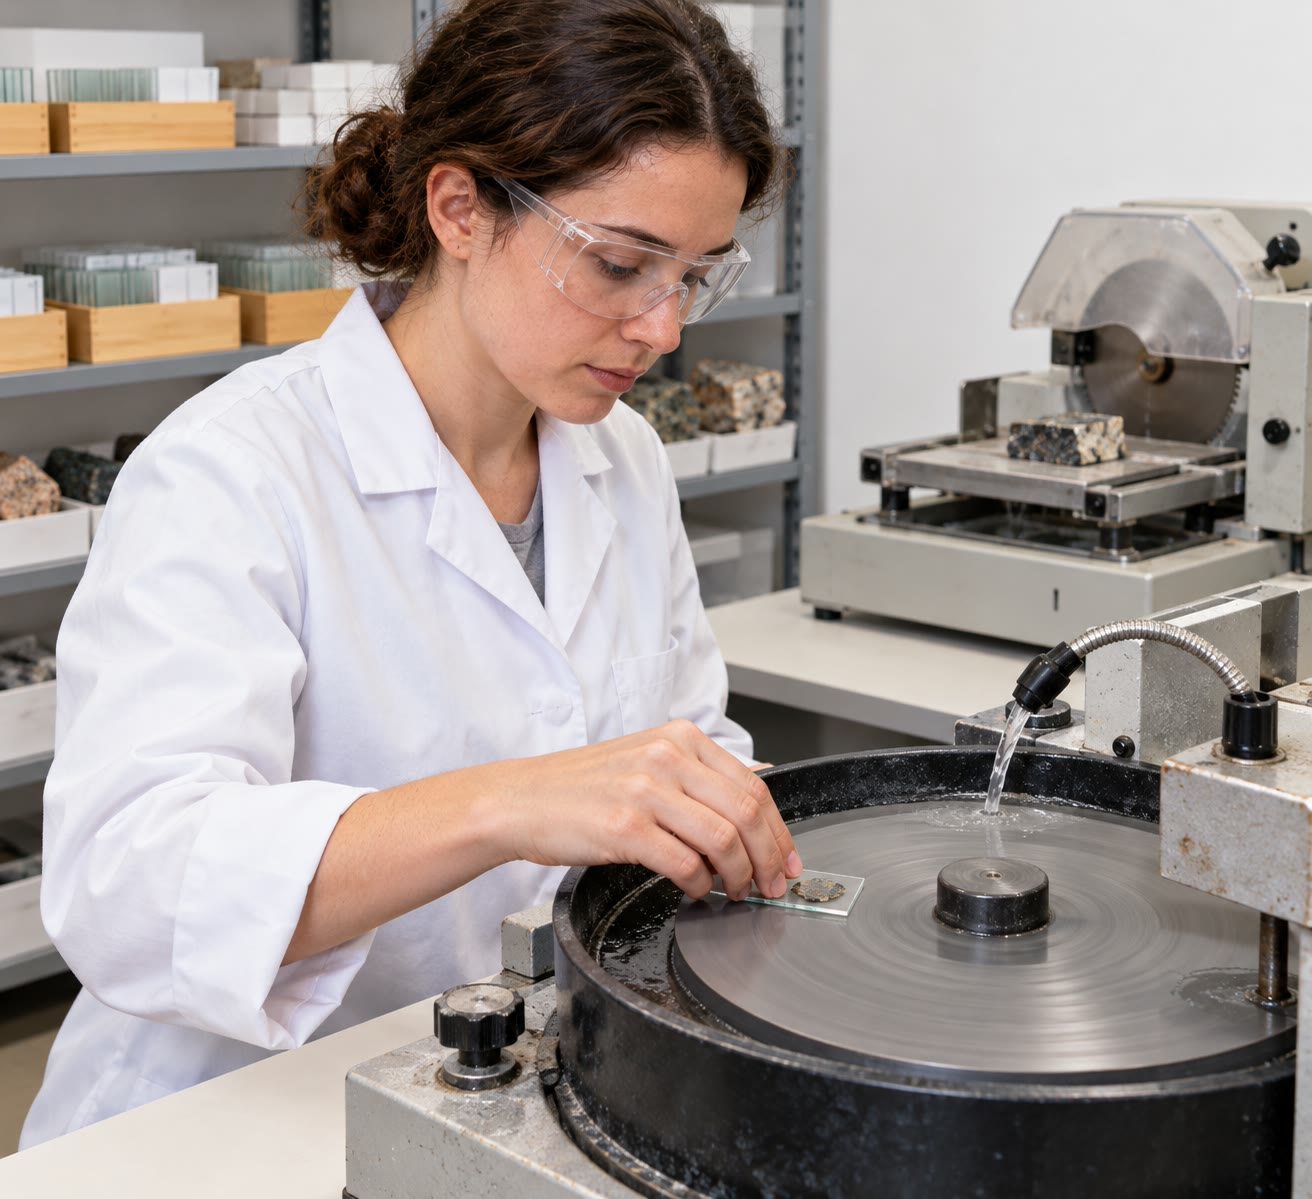
\includegraphics[width=\linewidth]{images/book3/ai/b1-thin-section-lab.jpg}
\end{minipage}
\end{inthelab}

La \omterm{def:b1:field-lab-methods-1:thin-section}{lámina delgada} se estudia con un microscopio provisto de dos filtros de polarización. La polarización
lineal es tema de la física: aquí basta con que un filtro de polarización solo deje pasar la luz que vibra
en una dirección, y que dos filtros colocados en ángulo recto no dejen pasar nada.

\begin{definition}[Microscopio de polarización, luz polarizada plana, nicoles cruzados]\label{def:b1:field-lab-methods-1:microscope}
Un \emph{microscopio de polarización}\index{microscopio de polarización} es un microscopio de luz transmitida
con un filtro de polarización (el polarizador) bajo una platina que gira \ang{360} frente a una escala
graduada, y un segundo filtro de polarización (el analizador) entre el objetivo y el ocular, que puede
moverse dentro o fuera del camino de la luz, con su dirección de vibración en ángulo recto con la del
polarizador. Con el analizador fuera, la muestra se ve en \emph{luz polarizada plana}\index{luz polarizada plana};
con el analizador dentro, se ve entre \emph{nicoles cruzados}\index{nicoles cruzados}.
\end{definition}

\begin{omfigure}
\begin{tikzpicture}[font=\scriptsize, x=1cm, y=0.62cm]
\def\comp#1#2#3{\draw[fill=#3] (-1.1,#1-0.18) rectangle (1.1,#1+0.18); \node[right] at (1.3,#1) {#2};}
\draw[omThm!60, line width=3pt, -{Stealth[length=3mm]}] (0,0.3) -- (0,10.6);
\draw[fill=yellow!40] (0,0) circle (0.3); \node[right] at (1.3,0) {lámpara};
\comp{1.3}{polarizador: transmite una dirección de vibración}{omDef!25}
\draw[omDef, thick, <->] (-0.5,1.3) -- (0.5,1.3);
\draw[fill=white] (-1.0,2.3) .. controls (0,2.75) .. (1.0,2.3) .. controls (0,1.85) .. (-1.0,2.3);
\node[right] at (1.3,2.3) {condensador};
\draw[fill=black!70] (-1.6,3.4) rectangle (1.6,3.55);
\draw[fill=icsJurassic!40] (-0.5,3.55) rectangle (0.5,3.65);
\node[right] at (1.7,3.48) {platina giratoria, graduada en grados, con la lámina delgada};
\draw[fill=white] (-0.45,4.5) rectangle (0.45,5.4); \node[right] at (1.3,4.95) {objetivo};
\comp{6.2}{ranura para accesorios}{black!10}
\comp{7.2}{analizador: dentro (nicoles cruzados) o fuera (luz polarizada plana)}{omDef!25}
\draw[omDef, thick, <->] (0,6.85) -- (0,7.55);
\comp{8.2}{lente de Bertrand (opcional)}{black!5}
\draw[fill=white] (-0.35,9.1) rectangle (0.35,10.0); \node[right] at (1.3,9.55) {ocular con hilos cruzados};
\end{tikzpicture}

{\small El camino de la luz en un \omterm{def:b1:field-lab-methods-1:microscope}{microscopio de polarización} (esquema, de abajo arriba). El polarizador
y el analizador vibran en ángulo recto (flechas dobles); sin nada entre ellos, los \omterm{def:b1:field-lab-methods-1:microscope}{nicoles cruzados} dan un
campo negro.}
\end{omfigure}

Entre \omterm{def:b1:field-lab-methods-1:microscope}{nicoles cruzados}, el vidrio del portaobjetos, la resina y cualquier mineral isótropo (uno cuyas
propiedades ópticas son iguales en todas las direcciones, como los cristales cúbicos) permanecen negros
cualquiera que sea la rotación de la platina. La mayoría de los minerales no son isótropos: cambian la
polarización de la luz que los atraviesa, y aparecen con colores de interferencia que cambian al girar la
platina y se extinguen cuatro veces en una vuelta completa. Por qué lo hacen, y cómo los colores y los
ángulos identifican un mineral, es el tema de \cref{ch:b1:optical-mineralogy}. Los minerales en \omterm{def:b1:field-lab-methods-1:thin-section}{lámina
delgada} se examinan normalmente con aumentos de unos $16\times$ a $400\times$.
% ledger: jaic:magnification

\begin{omfigure}
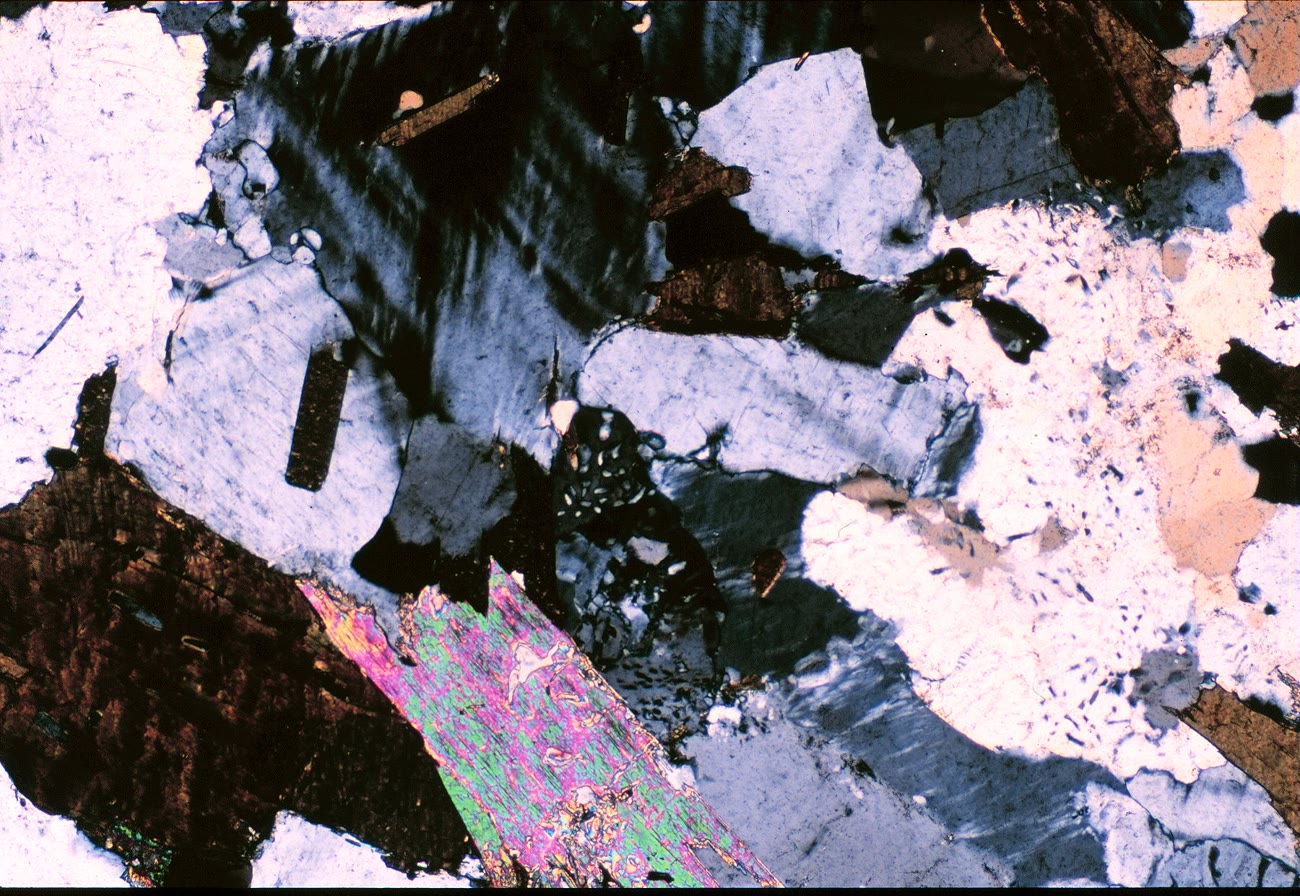
\includegraphics[width=0.55\linewidth]{images/book3/b1-granite-thin-section-xpl.jpg}
% ledger: commons:granite-xpl

{\small Un granito en \omterm{def:b1:field-lab-methods-1:thin-section}{lámina delgada} entre \omterm{def:b1:field-lab-methods-1:microscope}{nicoles cruzados}. La biotita es parda, la moscovita muestra
colores de interferencia rosas y verdes brillantes, la plagioclasa está rayada por sus maclas, y el cuarzo
es blanco o gris. Fotografía de Darla Sondrol, CC0 (Wikimedia Commons).}
\end{omfigure}

\begin{safety}
La práctica del campo y del laboratorio se hace segura con normas profesionales, no con la suerte.
En el campo, los geólogos trabajan por parejas o dejan por escrito su itinerario y la hora de regreso;
llevan la previsión del tiempo, mapas y primeros auxilios, se mantienen lejos del pie y del borde de
los acantilados y de los frentes de cantera, y usan casco y protección ocular allí donde la roca puede
caer o astillarse; el trabajo en lugares activos sigue las normas del operador. En el laboratorio, las
sierras y los discos trabajan protegidos por resguardos y con agua para reducir el polvo; las resinas y
los ácidos se manipulan con guantes y gafas bajo extracción, y cada producto químico tiene su ficha de
datos de seguridad. Ninguna de estas actividades es solo para un lector de este libro: el capítulo
describe la práctica profesional.
\end{safety}

\section{Ejercicios}

\begin{exercise}[$\star$]\label{exo:b1:field-lab-methods-1:1}
Un receptor de satélite da posiciones con unos \qty{4.9}{m} de error. ¿Cuánto es eso en un mapa a
1:10\,000? ¿Y a 1:25\,000?
\end{exercise}

\begin{exercise}[$\star$]\label{exo:b1:field-lab-methods-1:2}
Una brújula sin ajuste de declinación lee en un estrato la \omterm{def:b1:geological-maps:attitude}{dirección de buzamiento} \ang{052}. Dése la
\omterm{def:b1:geological-maps:attitude}{dirección de buzamiento} geográfica si la lectura se hizo en Reikiavik el 1 de enero de 2026, y después
en Wellington el mismo día (recuadro de datos).
\end{exercise}

\begin{exercise}[$\star$]\label{exo:b1:field-lab-methods-1:3}
Una recta de \omterm{def:b1:field-lab-methods-1:trend-plunge}{inmersión} \ang{20} hacia \ang{015}. Escríbase su orientación como en el texto, y dese su
vector unitario hacia abajo en componentes este, norte y arriba.
\end{exercise}

\begin{exercise}[$\star$]\label{exo:b1:field-lab-methods-1:4}
Tres lecturas de una diaclasa vertical dan los \omterm{def:b1:spherical-astronomy:horizontal}{acimutes} de su normal \ang{350}, \ang{358} y \ang{006}.
Calcúlese su media aritmética y después el \omterm{def:b1:spherical-astronomy:horizontal}{acimut} de la suma de los tres vectores unitarios horizontales.
¿Cuál de las dos medias es la correcta?
\end{exercise}

\begin{exercise}[$\star\star$]\label{exo:b1:field-lab-methods-1:5}
Cinco lecturas del \omterm{def:b1:geological-maps:attitude}{buzamiento} de un mismo estrato son \ang{34}, \ang{37}, \ang{35}, \ang{33} y \ang{36}.
Calcúlense su media, su desviación típica y el error típico de la media.
\end{exercise}

\begin{exercise}[$\star\star$]\label{exo:b1:field-lab-methods-1:6}
Un geólogo promedia una lectura en cada flanco de un \omterm{def:b1:geological-maps:fold}{pliegue} simétrico: $090/30$ y $270/30$.
Calcúlense la media vectorial y $\bar R$. ¿Qué ha salido mal?
\end{exercise}

\begin{exercise}[$\star\star$]\label{exo:b1:field-lab-methods-1:7}
Unas estrías sobre una superficie de estratificación de \omterm{def:b1:geological-maps:attitude}{actitud} $080/12$ tienen la \omterm{def:b1:field-lab-methods-1:trend-plunge}{dirección}
\ang{120}. ¿Cuál es su \omterm{def:b1:field-lab-methods-1:trend-plunge}{inmersión}? ¿Cuál sería para la \omterm{def:b1:field-lab-methods-1:trend-plunge}{dirección} \ang{170}?
\end{exercise}

\begin{exercise}[$\star\star$]\label{exo:b1:field-lab-methods-1:8}
En Edimburgo la declinación magnética es \ang{-0.47} el 1 de enero de 2026 y cambia \ang{+0.20} por año.
Suponiendo que el cambio sea constante, ¿cuándo se anula, y cuánto vale el 1 de enero de 2030?
\end{exercise}

\begin{exercise}[$\star\star$]\label{exo:b1:field-lab-methods-1:9}
Tres lecturas de un mismo estrato son $080/10$, $080/12$ y $080/14$. Demuéstrese que su media vectorial es
$080/12$, calcúlense $\bar R$ y la estimación $\sqrt{2(1 - \bar R)}$ de $\theta_{\text{rms}}$, y compárese
con el ángulo cuadrático medio exacto.
\end{exercise}

\begin{exercise}[$\star\star\star$]\label{exo:b1:field-lab-methods-1:10}
Una \omterm{def:b1:field-lab-methods-1:thin-section}{lámina delgada} corta un grano esférico de radio $r$ a una distancia $h$ de su centro, con $h$ igual
de probable en cualquier punto entre 0 y $r$. Demuéstrese que el radio medio del círculo que se ve en la
lámina es $\pi r/4$. ¿Qué tamaño medio aparece en la lámina un grano de cuarzo de \qty{0.50}{mm} de diámetro?
\end{exercise}

\begin{exercise}[$\star\star\star$]\label{exo:b1:field-lab-methods-1:11}
Demuéstrese que si a cada \omterm{def:b1:geological-maps:attitude}{dirección de buzamiento} de un conjunto de lecturas se le suma el mismo ángulo
$D$, la \omterm{def:b1:geological-maps:attitude}{dirección de buzamiento} de su media vectorial aumenta en $D$ y su \omterm{def:b1:geological-maps:attitude}{buzamiento} no cambia. ¿Por qué
importa esto para la corrección de la declinación?
\end{exercise}

\begin{exercise}[$\star\star\star$]\label{exo:b1:field-lab-methods-1:12}
Sobre un estrato que buza \ang{12}, la normal de una sola lectura se dispersa con una desviación típica de
\ang{2} en cada una de dos direcciones perpendiculares: a lo largo de la línea de máximo \omterm{def:b1:geological-maps:attitude}{buzamiento}, lo que
cambia el \omterm{def:b1:geological-maps:attitude}{buzamiento}, y a través de ella, lo que cambia la \omterm{def:b1:geological-maps:attitude}{dirección de buzamiento}. ¿Cuántas lecturas hacen
falta para un error típico de \ang{0.5} en el \omterm{def:b1:geological-maps:attitude}{buzamiento} medio? ¿Y de \ang{1} en la \omterm{def:b1:geological-maps:attitude}{dirección de buzamiento} media?
\end{exercise}

\section{Problema: una temporada de campo en el flanco oriental de Varden}

\begin{problem}[{Problema de fin de semana --- promediar doce lecturas de brújula, medir su dispersión,
corregirlas y compararlas con los sondeos}]
\label{pb:b1:field-lab-methods-1:1}
% readings: figdata/bachelor-1/attitude_stats.py (part normals); values: calc/ch06.py
Un geólogo midió la estratificación del flanco oriental del \omterm{def:b1:geological-maps:fold}{anticlinal} de Varden en doce estaciones, con
una brújula ajustada para la declinación, redondeando al grado. La tabla da cada lectura (\omterm{def:b1:geological-maps:attitude}{dirección de
buzamiento}/\omterm{def:b1:geological-maps:attitude}{buzamiento}) y las componentes de su normal unitaria hacia arriba $\vec n = (n_E, n_N, n_U)$,
redondeadas a cuatro decimales.
\begin{center}
\small
\begin{tabular}{rcccc@{\qquad}rcccc}
\hline
 & medida & $n_E$ & $n_N$ & $n_U$ & & medida & $n_E$ & $n_N$ & $n_U$ \\
\hline
1 & $076/11$ & 0.1851 & 0.0462 & 0.9816 & 7 & $083/11$ & 0.1894 & 0.0233 & 0.9816 \\
2 & $081/13$ & 0.2222 & 0.0352 & 0.9744 & 8 & $083/12$ & 0.2064 & 0.0253 & 0.9781 \\
3 & $078/16$ & 0.2696 & 0.0573 & 0.9613 & 9 & $085/12$ & 0.2071 & 0.0181 & 0.9781 \\
4 & $081/11$ & 0.1885 & 0.0298 & 0.9816 & 10 & $078/11$ & 0.1866 & 0.0397 & 0.9816 \\
5 & $076/10$ & 0.1685 & 0.0420 & 0.9848 & 11 & $081/13$ & & & \\
6 & $083/14$ & 0.2401 & 0.0295 & 0.9703 & 12 & $082/11$ & & & \\
\hline
\end{tabular}
\end{center}

\medskip
\noindent\textbf{Parte I --- La actitud media.}
\begin{enumerate}
  \item Calcúlense las medias aritméticas de las doce direcciones de \omterm{def:b1:geological-maps:attitude}{buzamiento} y de los doce \omterm{def:b1:geological-maps:attitude}{buzamientos}.
  \item Dé un ejemplo de dos lecturas para las que la media aritmética de las direcciones de \omterm{def:b1:geological-maps:attitude}{buzamiento} es
        absurda, y diga por qué aquí es segura.
  \item Demuéstrese que $\vec n = (\sin\delta\sin\alpha, \sin\delta\cos\alpha,
        \cos\delta)$ es un vector unitario perpendicular a la línea de máximo \omterm{def:b1:geological-maps:attitude}{buzamiento} y a la
        línea de \omterm{def:b1:geological-maps:attitude}{rumbo} del plano $\alpha/\delta$.
  \item Complétese la tabla para las lecturas 11 y 12.
  \item Calcúlese la resultante $\vec S$ de las doce normales.
  \item Calcúlense $\|\vec S\|$ y la longitud resultante media $\bar R$.
  \item Dedúzcase la media vectorial: su \omterm{def:b1:geological-maps:attitude}{dirección de buzamiento} y su \omterm{def:b1:geological-maps:attitude}{buzamiento}.
\end{enumerate}

\medskip
\noindent\textbf{Parte II --- La dispersión.}
\begin{enumerate}[resume]
  \item Calcúlense las desviaciones típicas muestrales de las direcciones de \omterm{def:b1:geological-maps:attitude}{buzamiento} y de los \omterm{def:b1:geological-maps:attitude}{buzamientos}.
  \item Con \cref{prop:b1:field-lab-methods-1:vector-mean}, estímese el ángulo cuadrático medio
        $\theta_{\text{rms}}$ entre las lecturas y su media, en grados.
  \item Prevea $\theta_{\text{rms}}$ a partir de las dos desviaciones típicas de la pregunta 8 y de la fórmula
        de error del capítulo, y compárese.
  \item ¿Cuál de las dos desviaciones típicas contribuye más a $\theta_{\text{rms}}$, y por qué?
  \item Calcúlense los errores típicos del \omterm{def:b1:geological-maps:attitude}{buzamiento} medio y de la \omterm{def:b1:geological-maps:attitude}{dirección de buzamiento} media.
  \item ¿Es la dispersión de las direcciones de \omterm{def:b1:geological-maps:attitude}{buzamiento}, \ang{2.9}, señal de una medida descuidada?
        Explíquese.
\end{enumerate}

\medskip
\noindent\textbf{Parte III --- La declinación.}
\begin{enumerate}[resume]
  \item Un segundo geólogo olvidó ajustar la declinación. Sus doce lecturas tienen como media vectorial
        $083.1/12.1$ en \omterm{def:b1:spherical-astronomy:horizontal}{acimutes} magnéticos. Supóngase que la declinación magnética en las colinas de Varden ese
        año es de \ang{2.5} oeste. ¿Cuál es su media en \omterm{def:b1:spherical-astronomy:horizontal}{acimutes} geográficos?
  \item ¿Por qué su \omterm{def:b1:geological-maps:attitude}{buzamiento} medio es correcto sin corrección?
  \item ¿Podría haber corregido cada lectura antes de promediar, en lugar de la media? ¿Cambia la respuesta
        (\cref{exo:b1:field-lab-methods-1:11})?
  \item Diez años después, un estudiante reutiliza su ajuste de declinación mientras la declinación ha
        cambiado \ang{0.2} por año. ¿Cuánto vale el error, comparado con el error típico de la pregunta 12?
  \item Dé el \omterm{def:b1:geological-maps:attitude}{rumbo} de la \omterm{def:b1:geological-maps:attitude}{actitud} media del primer geólogo según la regla de la mano derecha.
\end{enumerate}

\medskip
\noindent\textbf{Parte IV --- Brújula y sondeos.}
\begin{enumerate}[resume]
  \item A partir de tres sondeos, \cref{ch:b1:geological-maps} halló para la base de la caliza la \omterm{def:b1:geological-maps:attitude}{actitud}
        $080.6/12.2$. Compárese con la media vectorial de la pregunta 7, ángulo a ángulo.
  \item Calcúlese el ángulo entre las dos normales.
  \item El error típico de la \omterm{def:b1:field-lab-methods-1:trend-plunge}{dirección} media es aproximadamente $\theta_{\text{rms}}/\sqrt N$. ¿Es
        significativa la diferencia de la pregunta 20?
  \item ¿Cuántas lecturas reducirían a la mitad ese error típico?
  \item Nombre dos errores que ningún número de lecturas reduciría.
  \item Dé la \omterm{def:b1:geological-maps:attitude}{actitud} media del flanco oriental a partir de las doce lecturas, en la forma \omterm{def:b1:geological-maps:attitude}{dirección de
        buzamiento}/\omterm{def:b1:geological-maps:attitude}{buzamiento} redondeada al grado.
\end{enumerate}
\end{problem}
